\subsection{Stack pivoting}
Stack Pivoting is a technique used when facing lack space on the stack - for
example, when the buffer overflow allow only to overwrite the \verb+ip+. In this scenario, it is not possible to complete a full ROP chain.

During Stack Pivoting, the shellcode take control of the RSP register and
"fake" the location of the stack. There are a few ways to do this.

\url{https://ir0nstone.gitbook.io/notes/types/stack/stack-pivoting}

\subsubsection{sub esp pivoting}
Consider the following example
\begin{verbatim}
void buy(void)
{
  undefined auStack_48 [72];

  read(0,auStack_48,0x58);
  return;
}
\end{verbatim}

and consider the assembly code is the following with no \verb+push/pop rbp+ (strange but happen)

\begin{verbatim}
   0x55555555532a:      sub    rsp,0x48
   0x555555555348:      mov    rsi,rsp
   0x55555555534b:      mov    edx,0x50
   0x555555555350:      xor    edi,edi
   0x555555555352:      call   0x555555555060 <read@plt>
   0x555555555357:      add    rsp,0x48
   0x55555555535b:      ret
\end{verbatim}


The payload is only able to overwrite the \verb+ip+ but with with the help of a
\verb+sub rsp+ ROP gadget it is possible to increase the size of the stack and
place it a ROP chain.


considering the following 
\begin{verbatim}
$ ropper --file binary --search sub
[INFO] Load gadgets from cache
[LOAD] loading... 100%
[LOAD] removing double gadgets... 100%
[INFO] Searching for gadgets: sub

[INFO] File: pwnshop
0x000000000000121a: sub esp, 0x28; ret;
0x00000000000013dd: sub esp, 8; add rsp, 8; ret;
0x0000000000001005: sub esp, 8; mov rax, qword ptr [rip + 0x2fd9]; test rax, rax; je 0x1016; call rax;
\end{verbatim}



 \begin{figure}
     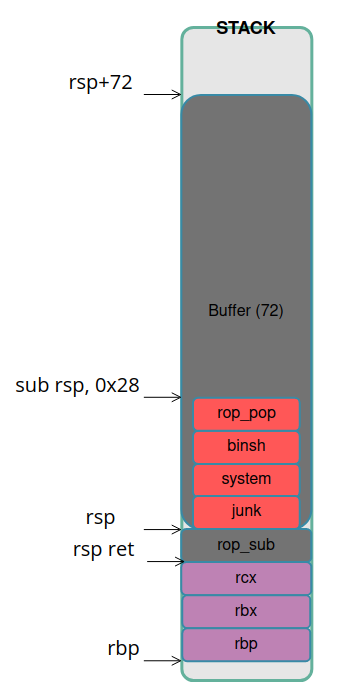
\includegraphics[width=.5\linewidth]{binary/exploit_linux/images/sub_rsp_pivoting.png}
  \caption{Registry parts}
  \label{fig:sub_rsp_pivoting}
\end{figure}
